% !TEX root = ../../main.tex
% !TEX spellcheck = en_GB
\section{Design}
The design of the MATLAB framework is shown in \cref{fig:classbdd}.

\paragraph{The TransferFunction class} implements the \mintinline{matlab}{plotResponse(f)} method, and the  abstract method \mintinline{matlab}{transform(x)}.
\mintinline{matlab}{plotResponse(f)} plots the amplitude spectrum in the range given by the argument \mintinline{matlab}{f}.
It uses the implemented, by any subclass, \mintinline{matlab}{transform(x)} method to access the frequency response.

\begin{figure}
	\centering
	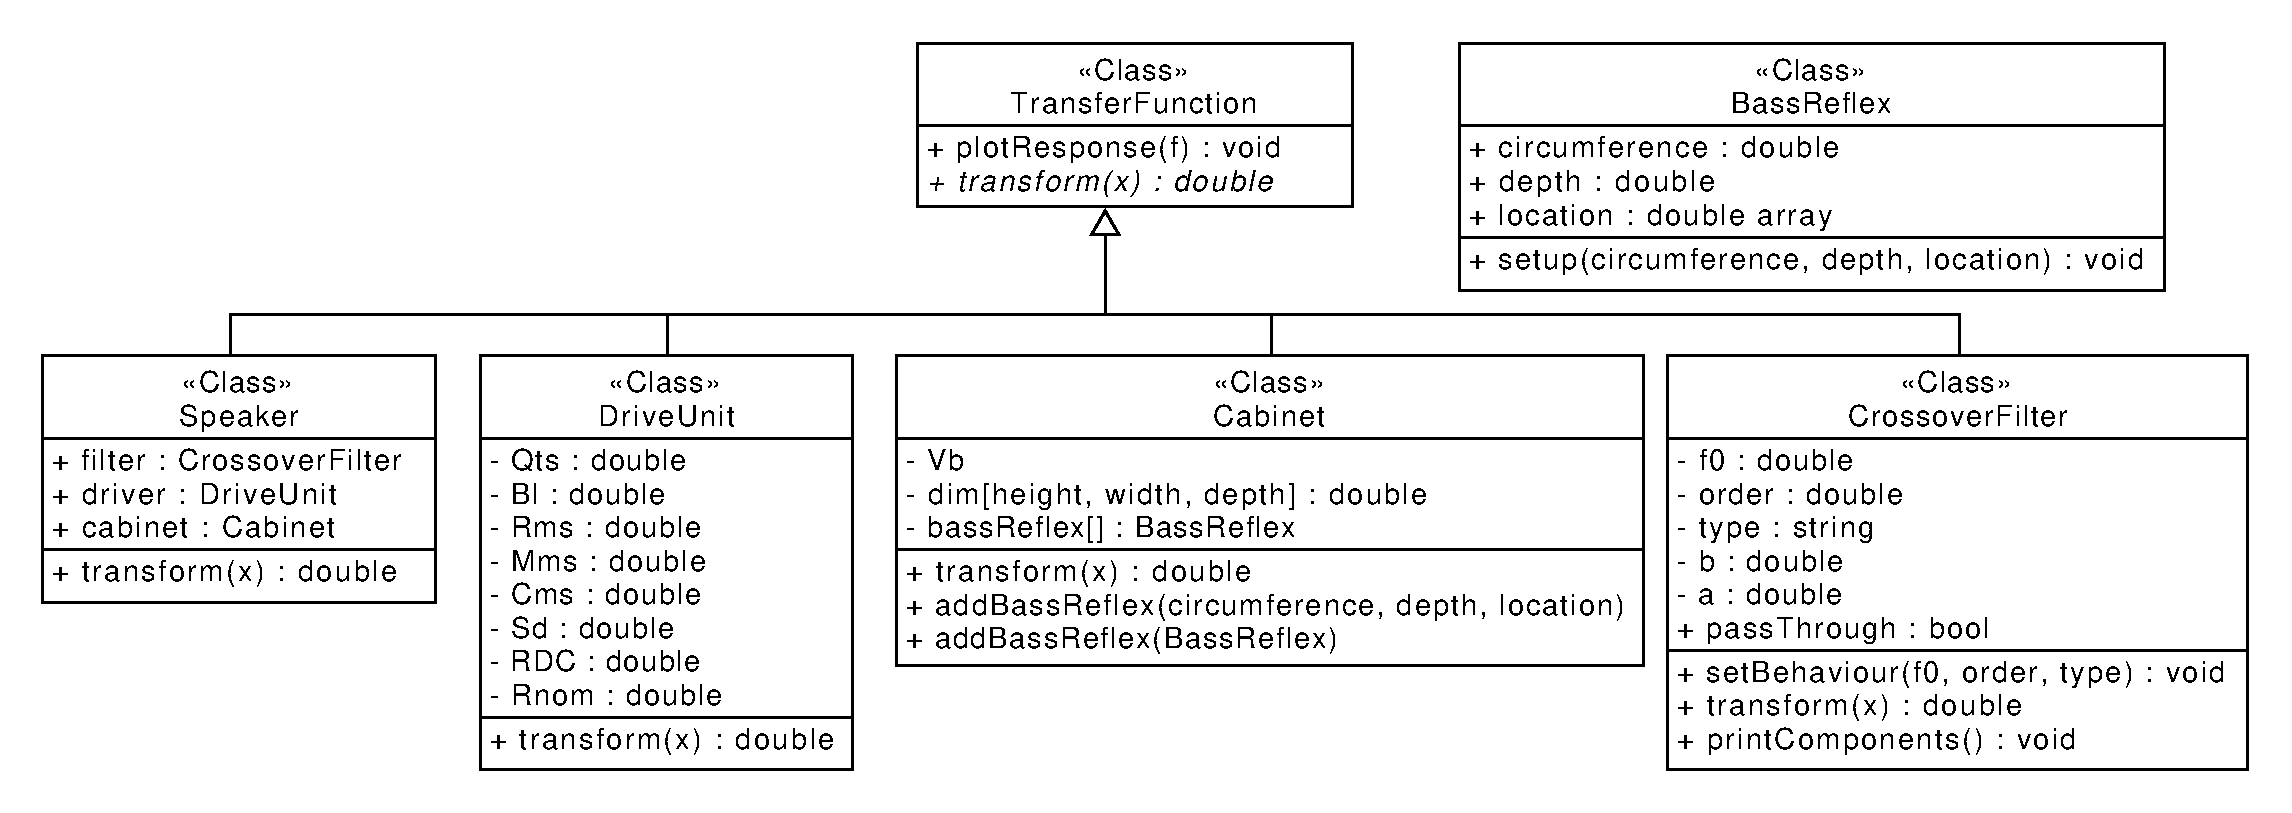
\includegraphics[width=\linewidth]{gfx/Design/Class_BDD}
	\caption{Class diagram of the MATLAB framework.}
	\label{fig:classbdd}
\end{figure}

\paragraph{The Speaker class} contains the objects necessary to calculate the transfer function for the complete speaker.
It's purpose is to collect the other units, to test them together, and to provide the frequency response to compare with the measured response.

\paragraph{The DriveUnit class} describes the drive unit on the basis of Thiele/Small parameters\cite{thielesmall} and \cref{eq:transdriveunit} \cite[p.~41]{Elektroakustik}.
The \mintinline{matlab}{plotResponse(f)} function plots the response of the drive unit in an infinitely large closed box.

\begin{equation}
	p = \frac{\rho S_D B l U_G}{2\pi r M_{MS} R_E}\left|\frac{s^2}{s^2 + \frac{\omega_s}{Q_{TS}}s+\omega_s^2}\right|
	\label{eq:transdriveunit}
\end{equation}

\paragraph{The Cabinet class} describes a closed box cabinet, with the possibility to add a number of bass reflexes and check if their locations are valid.
Without bass reflexes \mintinline{matlab}{plotResponse(f)} plots the response in a cabinet of the specified volume, according to \cref{eq:dutfclosed}.
If bass reflexes are present, it should plot the frequency response according to \fxnote{Ref to eqs.}

\paragraph{The CrossoverFilter class} is meant to filter the input before it reaches the physical parts of the speaker.
It is meant to either be used to filter the signal in an appropriate way if several drive units are installed, or to try to refine the signal, if the speaker response is not satisfactory.

\paragraph{The BassReflex class} is a bass reflex tube placed somewhere on the cabinet.
It cannot itself show a frequency response, but must be placed in a cabinet.